\section{Results}
\label{sec:results}

\subsection{Participants and valid data}
All 24 participants completed both sessions, so all 48 scheduled sessions took place, and every one matched the frozen schedule and the SHA-256-locked WA manifests (\texttt{full\_analysis.ipynb}, Section 1).
The planned sample was 48 participants with a minimum of 24, so, following the protocol, this study is reported as exploratory.
Two participants were excluded from the paired analysis because their PITest session ended with an After suite that did not compile at T = 20 minutes (failure type \textit{method}); their JaCoCo sessions were excluded with them.
This leaves N = 22 of 24 participants (91.7\%) in the main analysis (Table~\ref{tab:excluded}).
Two PITest sessions started from a Before suite that did not compile (one of them is SV14-1 above); following the protocol, such sessions are kept with WADR(Before) = 0.

\subsection{RQ1: J versus P}
\textbf{RQ1.} Within the same time budget, how do uncovered-branch feedback from JaCoCo (condition J) and surviving-mutant feedback from PITest (condition P) differ in the gain in detection rate of held-out Wrong Answer submissions, relative to the participant's own initial JUnit suite?
$H_0$: $\theta$ = 0; $H_1$: $\theta$ $\neq$ 0, where $\theta$ is the pseudo-median of d = $\Delta$WADR(P) - $\Delta$WADR(J).

\textit{Descriptive statistics.}
In condition J, $\Delta$WADR had a median of 0.044 (IQR 0.000 to 0.198, range 0.000 to 0.750, 24 sessions); in condition P, the median was 0.000 (IQR 0.000 to 0.225, range $-$0.130 to 0.667, 22 sessions) (Table~\ref{tab:main}, Fig.~\ref{fig:dist}).
$\Delta$WADR was zero in 9 of 24 J sessions and 11 of 22 P sessions, and negative in one P session.
Across the 22 participants, the paired difference d had a median of $-$0.005 (IQR $-$0.174 to 0.061); 7 participants had $d > 0$, 11 had $d < 0$ and 4 had $d = 0$.
The distribution of d showed no strong asymmetry (skewness 0.26; Fig.~\ref{fig:dist}, right).

\textit{Test and effect size.}
The two-sided Wilcoxon signed-rank test (Pratt treatment of zeros, normal approximation because of zero differences) gave W = 100, p = 0.483.
The Hodges--Lehmann estimate was $\hat{\theta}$ = $-$0.012 with a 95\% confidence interval of [$-$0.118, 0.074], and the matched-pairs rank-biserial correlation was r = $-$0.16 (small).
Since p $\geq$ 0.05 and $|\hat{\theta}| < \delta$ = 0.10, we fail to reject $H_0$: no difference between J and P was found for RQ1.
The interval includes differences as large as 0.12 in favour of JaCoCo and 0.07 in favour of PITest.

\subsection{Pre-specified supplementary and sensitivity analyses}
All analyses specified in the protocol led to the same conclusion as the main analysis (Table~\ref{tab:sens}).
Counting an After suite that does not compile as WADR = 0 (N = 24) gave $\hat{\theta}$ = $-$0.016, p = 0.350.
Using T = 15 or T = 30 minutes gave $\hat{\theta}$ between $-$0.016 and 0.000 with p $\geq$ 0.350.
A linear mixed model with condition, session order and problem as fixed effects and participant as a random effect estimated the effect of P at $-$0.010 (95\% CI [$-$0.101, 0.081], p = 0.829; 46 sessions); adding the number of independent inputs or WADR(Before) as covariates gave $-$0.028 and $-$0.010.
In the 2$\times$2 crossover regression, the order-adjusted effect was $-$0.021 ([$-$0.130, 0.089]) and the period effect was 0.004 (p = 0.934).
The conclusion did not change when we kept all tests that disagreed with the reference Accepted solutions, when we counted WA submissions detected through an exception (secondary measure), or when we dropped participants whose problem had more items that the reference inputs could not cover or kill than items they could (N = 10).
The conclusion was also the same with $\delta$ = 0.05 and $\delta$ = 0.15.
In the subgroups below and above the median initial WADR (11 participants each), $\hat{\theta}$ was $-$0.016 and $-$0.001 (both p $\geq$ 0.27).
Per-problem means of $\Delta$WADR are shown in Fig.~\ref{fig:problem}; each problem had one or two sessions per condition, so no per-problem tests were run.

\textit{Feedback received.} JaCoCo produced a report in all 96 tool runs (24 sessions $\times$ 4 runs).
PITest produced a report in 30 of 96 runs (12 of 24 first runs); in 58 runs it stopped because at least one test failed on the program under test, and in 8 runs the suite did not compile.
In an exploratory analysis restricted to the 11 participants whose PITest session received at least one report, $\hat{\theta}$ = $-$0.020 ([$-$0.212, 0.180], p = 0.623).
No session reached the ceiling in condition J (WADR(After) $\geq$ 0.95 in 0 of 24), and one did in condition P (1 of 22).
Three tests in one JaCoCo session disagreed with the reference Accepted solutions; WADR was the same whether they were kept or removed.

\begin{table}[t]
\centering
\caption{RQ1: $\Delta$WADR at $T = 20$ minutes by condition and the paired comparison ($N = 22$ participants).}
\label{tab:main}
\begin{tabular}{lccccc}
\hline
 & Sessions & Median (IQR) & $p$ & $\hat{\theta}$ [95\% CI] & $r$ \\
\hline
J (JaCoCo) & 24 & 0.044 (0.000--0.198) & & & \\
P (PITest) & 22 & 0.000 (0.000--0.225) & & & \\
$d = P - J$ & 22 pairs & $-0.005$ ($-0.174$--$0.061$) & \textbf{0.483} & \textbf{$-0.012$ [$-0.118$, $0.074$]} & $-0.16$ \\
\hline
\end{tabular}
\end{table}

\begin{table}[t]
\centering
\caption{Sensitivity and supplementary analyses for RQ1. Rows marked $^{\dagger}$ are exploratory.}
\label{tab:sens}
\begin{tabular}{lccc}
\hline
Analysis & $N$ & $\hat{\theta}$ [95\% CI] & $p$ \\
\hline
Main ($T = 20$, non-compiling After excluded) & 22 & $-0.012$ [$-0.118$, $0.074$] & 0.483 \\
Non-compiling After counted as 0 & 24 & $-0.016$ [$-0.126$, $0.063$] & 0.350 \\
$T = 15$ & 23 & $0.000$ [$-0.090$, $0.141$] & 0.927 \\
$T = 30$ & 22 & $-0.012$ [$-0.129$, $0.074$] & 0.504 \\
Keep tests disagreeing with Accepted solutions & 22 & $-0.012$ [$-0.118$, $0.074$] & 0.483 \\
Secondary measure (exception counts as detection) & 22 & $-0.019$ [$-0.130$, $0.074$] & 0.407 \\
Drop problems with many unreachable report items & 10 & $-0.005$ [$-0.189$, $0.083$] & 0.716 \\
Mixed model, coefficient of P (sessions) & 46 & $-0.010$ [$-0.101$, $0.081$] & 0.829 \\
Crossover regression, order-adjusted & 22 & $-0.021$ [$-0.130$, $0.089$] & 0.700 \\
Participants with $\geq 1$ PITest report$^{\dagger}$ & 11 & $-0.020$ [$-0.212$, $0.180$] & 0.623 \\
\hline
\end{tabular}
\end{table}

\begin{figure}[t]
\centering
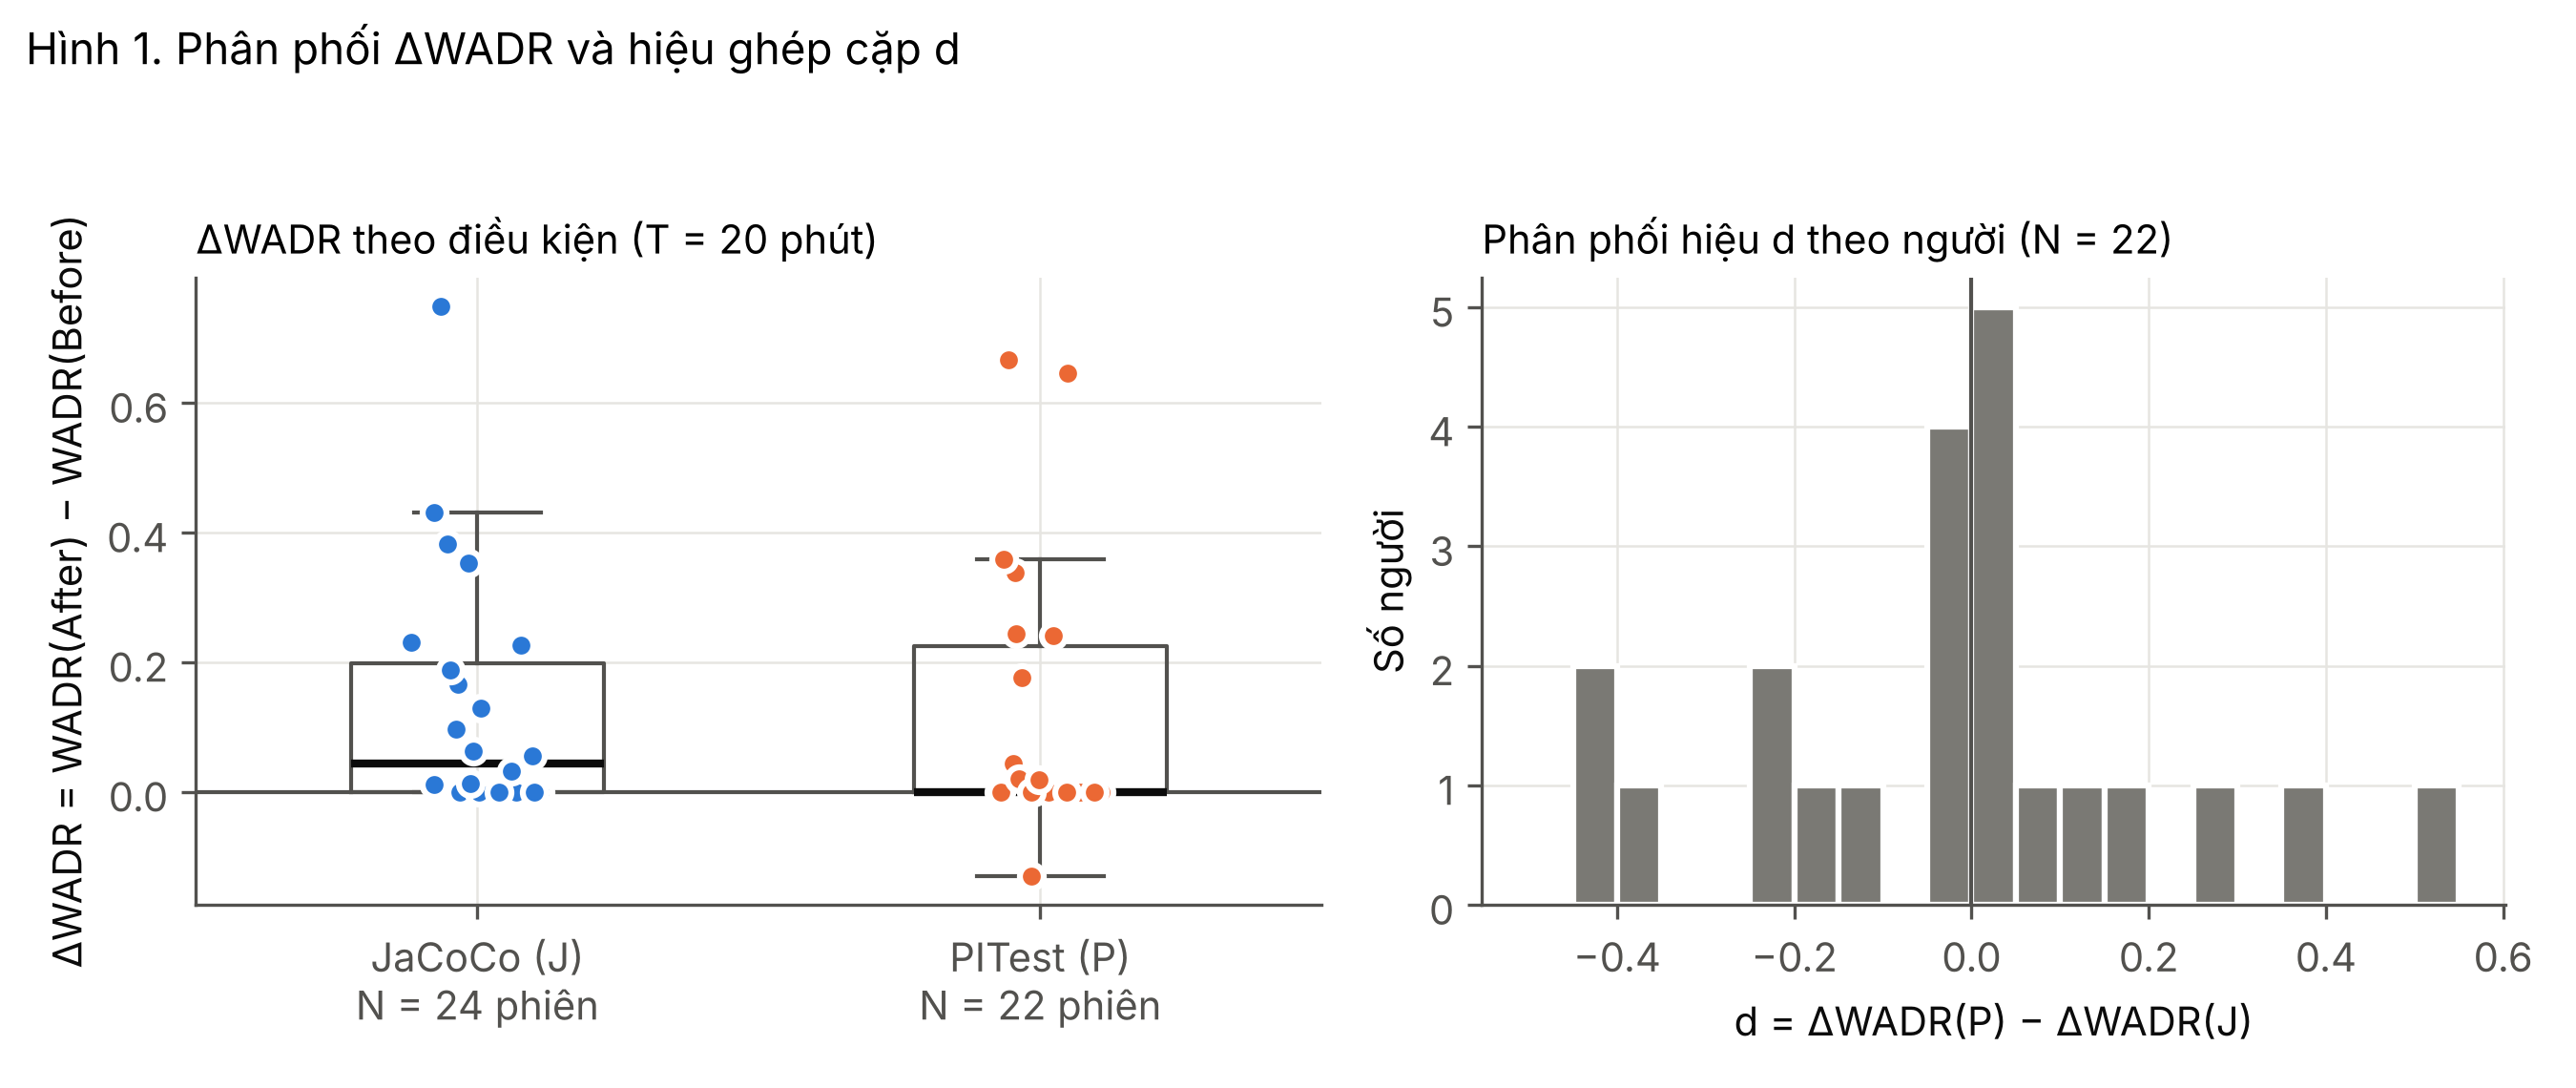
\includegraphics[width=\linewidth]{figures/fig1_distribution.png}
\caption{Left: $\Delta$WADR at $T = 20$ by condition (J: 24 sessions, P: 22 sessions). Right: paired difference $d$ per participant ($N = 22$).}
\label{fig:dist}
\end{figure}

\begin{figure}[t]
\centering
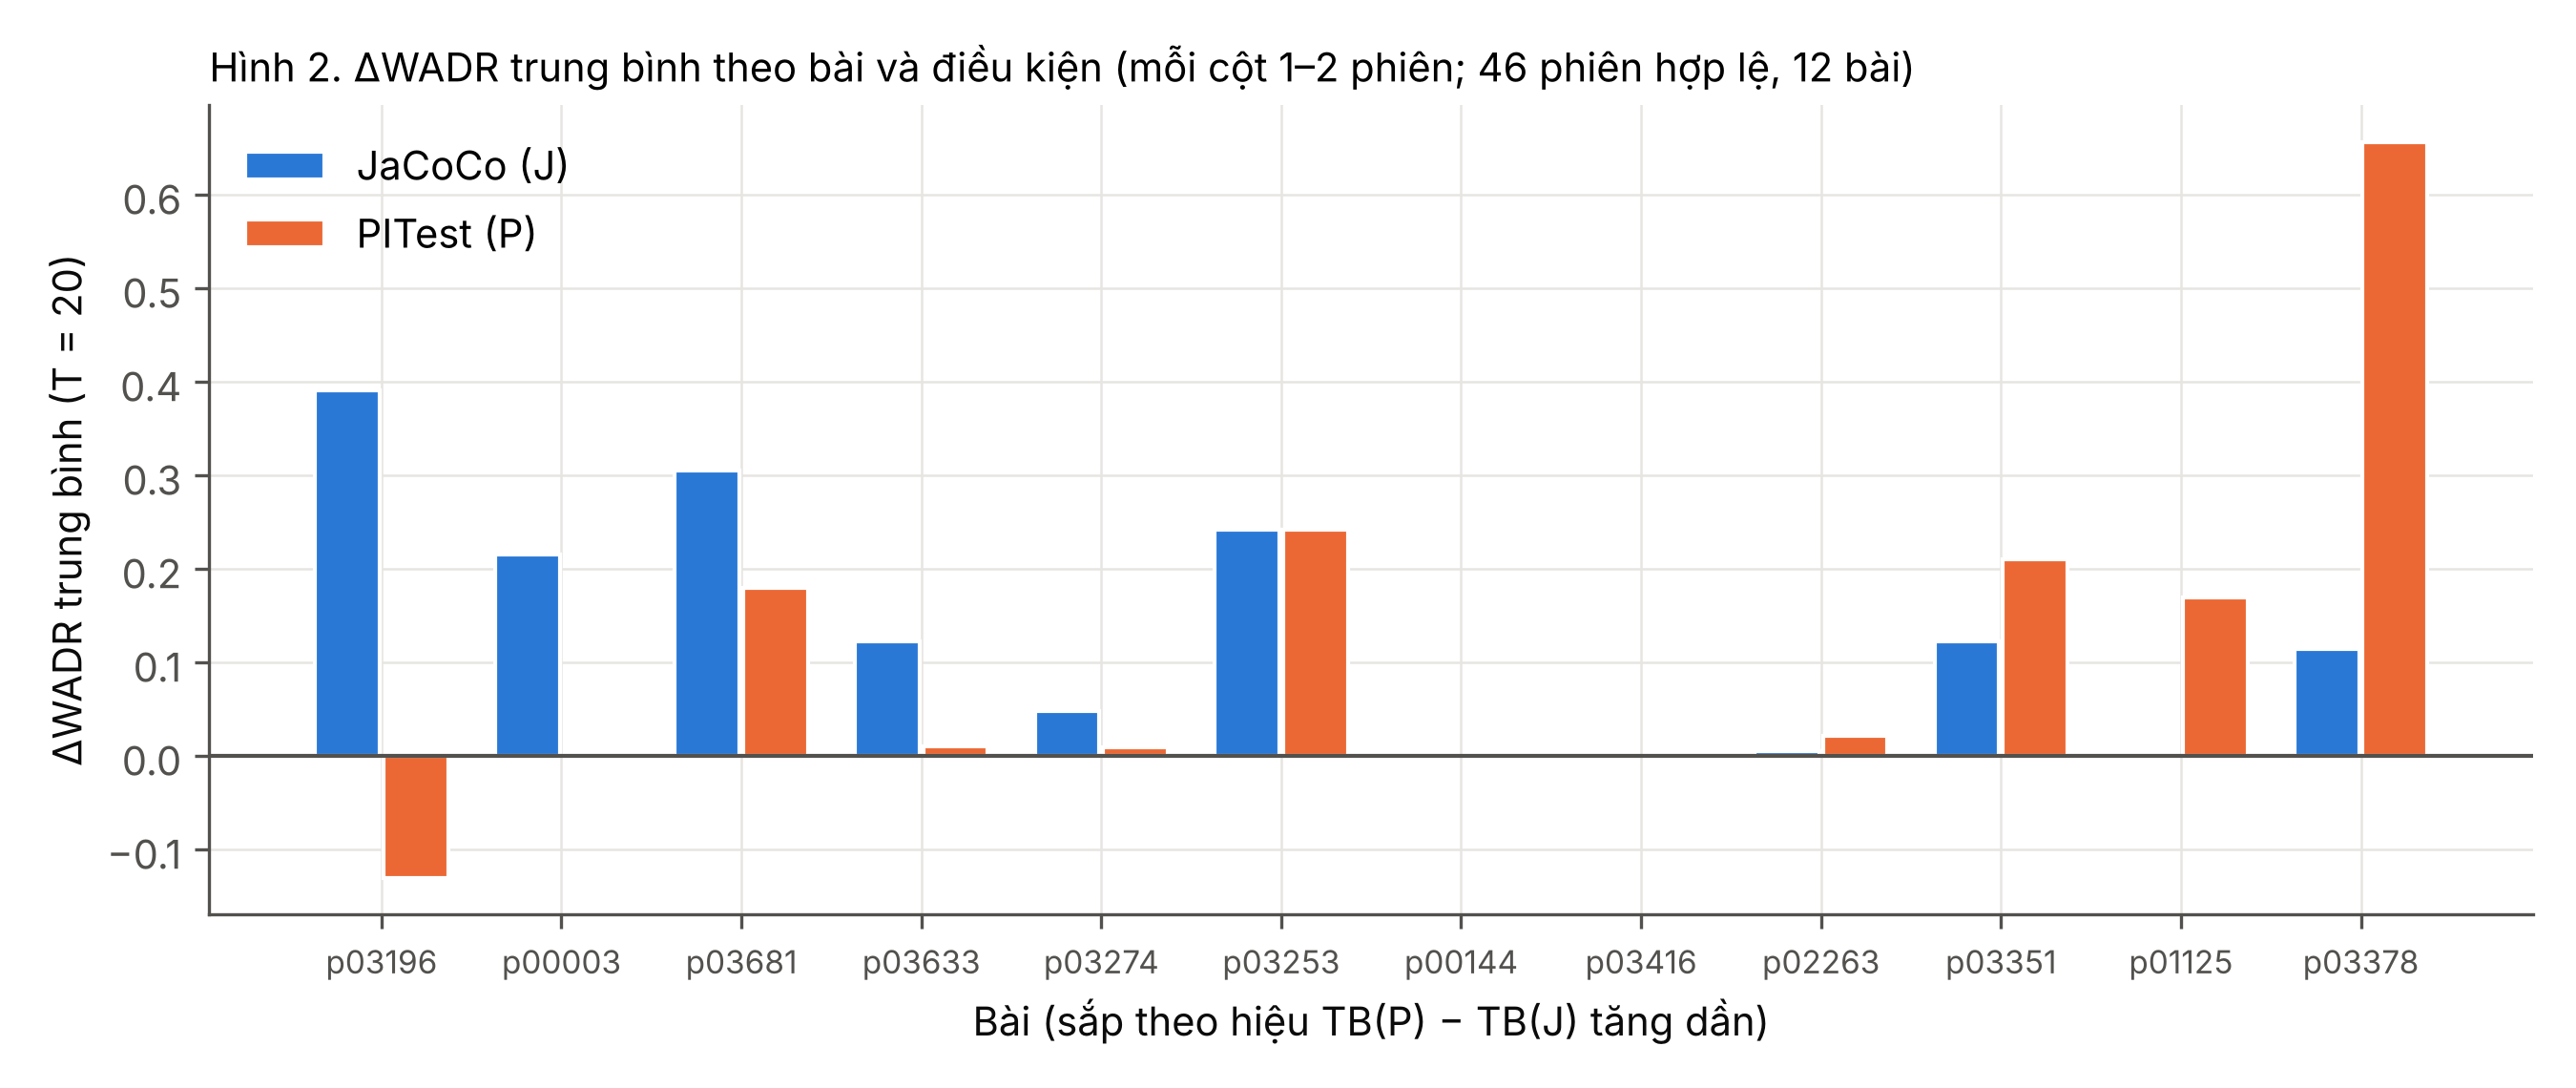
\includegraphics[width=\linewidth]{figures/fig2_comparison.png}
\caption{Mean $\Delta$WADR at $T = 20$ per problem and condition (one or two sessions per bar; 46 valid sessions, 12 problems).}
\label{fig:problem}
\end{figure}

\begin{table}[t]
\centering
\caption{Sessions excluded from the main paired analysis (\texttt{results/excluded.csv}).}
\label{tab:excluded}
\begin{tabular}{llll}
\hline
Session & Condition & Failure type & Reason \\
\hline
SV14-1 & P & method & After ($T = 20$) does not compile \\
SV14-2 & J & -- & partner session excluded \\
SV24-1 & P & method & After ($T = 20$) does not compile \\
SV24-2 & J & -- & partner session excluded \\
\hline
\end{tabular}
\end{table}

